% Beamer presentation
\documentclass[11pt,aspectratio=43,ignorenonframetext,t]{beamer}

% Presentation settings
\mode<presentation>{
  \usetheme[framenumber,titleframestart=1]{UoM_alex}
  \usefonttheme{professionalfonts} % using non standard fonts for beamer
  \usefonttheme{serif}
  \usepackage{fontspec}
  \setmainfont[Ligatures=TeX]{Arial}
}

% Handout settings
\mode<article>{
  \usepackage{fullpage}
  \usepackage{fontspec}
  \setmainfont[Ligatures=TeX]{Arial}
  \setlength{\parskip}{1.5\baselineskip} % correct beamer line spacings
  \setlength{\parindent}{0cm}
  \usepackage{enumitem}
  \setlist[itemize]{topsep=0pt}
}

 % Packages
\usepackage{graphicx}
\graphicspath{{./images/png}} % generic graphics path; overridden if necessary
\usepackage{amsmath}
\allowdisplaybreaks[1] % allow eqnarrays to break across pages
\usepackage{amssymb} 
\usepackage[HTML]{xcolor}
\definecolor{uomlinkblue}{HTML}{0071BC}
\usepackage{hyperref}
\hypersetup{
  colorlinks=true,
  linkcolor=uomlinkblue,
  filecolor=uomlinkblue,      
  urlcolor=uomlinkblue,
  pdflang={en-GB},
}
\usepackage[document]{ragged2e} % left aligned text for accessibility
\usepackage{tikz}
\usetikzlibrary{positioning, arrows, arrows.meta}
\usepackage{unicode-math} % unicode maths for accessibility
\usepackage{pdfcomment}   % for alt text for accessibility
\usepackage{rotating}     % allow portrait figures and tables
\usepackage{subfigure}    % allow matrices of figures
\usepackage{float}        % allows H option on floats to force here placement
\usepackage{multirow}     % allows merging of rows in tables
\usepackage{tabularx}     % allows fixed width tables
\usepackage{ctable}       % modifies \hline for use in table
\usepackage{bm}           % allow bold fonts in equations
\usepackage{pgf}          % allow graphics manipulation
\usepackage{etoolbox}
  
% Custom commands
\newcolumntype{Z}{>{\centering\arraybackslash}X}  % tabularx centered columns 

\makeatletter
  \DeclareRobustCommand{\em}
  {
    \@nomath\em
    \if b
      \expandafter\@car\f@series\@nil \normalfont
    \else
      \bfseries
    \fi
  }
\makeatother

\makeatletter
  \preto{\@verbatim}{\topsep=0pt \partopsep=0pt}
\makeatother

\def\checkmark{
  \tikz\fill[scale=0.4](0,.35) -- (.25,0) -- (1,.7) -- (.25,.15) -- cycle;
}

% Counters
\newcounter{example_number} % keep track of the example questions

% Frontmatter
\newcommand{\cmclecture}[1]{
  \title{Combinatorial Mesh Calculus (CMC): Lecture #1}
}
\author{
  Lectured by:
  \href{https://scholar.google.com/citations?user=x4R-snQAAAAJ&hl=en}
  {Dr. Kiprian Berbatov}$^1$\\
  \smallskip
  Lecture Notes Compiled by:
  \href{https://scholar.google.com/citations?user=CoIpITkAAAAJ&hl=en}
  {Muhammad Azeem}$^1$\\
  \smallskip
  Under the supervision of:
  \href{https://scholar.google.co.uk/citations?user=3nWJe5wAAAAJ&hl=en}
  {Prof. Andrey P. Jivkov}$^1$\\
  \smallskip
  {\tiny $^1$Department of Mechanical and Aerospace Engineering,
    The University of Manchester, Oxford Road, Manchester M13 9PL, UK}
}

% Special frames
\newcommand{\cmctitleframe}{
  \titlepage
  \begin{tikzpicture}[remember picture,overlay]
    \node[anchor=south east] at (current page.south east) {
      \href{https://youtube.com/@kipi.berbatov}{
        \includegraphics[width=1.5cm]{youtube-icon.png}
      }
    };
  \end{tikzpicture}
}
\newcommand{\cmcendframe}{
  \begin{figure}
    \centering
    \includegraphics[width=0.85\linewidth]{Thanks.png}
  \end{figure}
}

\cmclecture{5}
\date{20 October 2025}

\begin{document}

%========================= TITLE =========================
\begin{frame}
  \cmctitleframe
\end{frame}

\begin{frame}{Dimension}
Let $R$ be a commutative ring with unity (CRWU), and let $V$ be an $R$–module.

\begin{block}{Definitions}
\begin{itemize}
  \item $V$ is \textbf{free} if it has a basis, i.e.\ a subset $E\subseteq V$ such that every $v\in V$ can be written uniquely as a finite $R$–linear combination of elements of $E$.
  \item $V$ is \textbf{finite–dimensional} if it has a finite basis.
  \item If $E=\{e_1,\dots,e_n\}$ is a basis of $V$, we write $\dim_E V = n$.
\end{itemize}
\end{block}

\textbf{Remarks:} Free modules generalize vector spaces when the underlying field is replaced by a ring. The existence of a basis ensures that every element can be expressed uniquely in terms of simple building blocks.

\end{frame}


\begin{frame}{Well–defined dimension for free modules}


\begin{block}{Theorem }
Let $R$ be a CRWU and $V$ a finite-dimensional $R$–module. If $E$ and $F$ are bases of $V$, then
\[
\dim_E V = \dim_F V.
\]
We therefore denote the unique value by $\dim V$ and call it the \emph{rank} of $V$.
\end{block}
\textbf{Proof}
It suffices to show: if $R^m \cong R^n$ as $R$–modules, then $m=n$.
Indeed, a finite-dimensional module $V$ with a basis of size $m$ is isomorphic to $R^m$, so any two bases yield $R^m \cong R^n$.

Let $\mathfrak m$ be a maximal ideal of $R$; then $k:=R/\mathfrak m$ is a field. Tensoring the isomorphism $R^m \cong R^n$ with $k$ over $R$ gives
\[
k \otimes_R R^m \;\cong\; k \otimes_R R^n.
\]
\end{frame}

\begin{frame}{Proof (Continue) }
\begin{block}{}
Since $k\otimes_R R \cong k$ and tensor commutes with finite direct sums,
\[
k \otimes_R R^m \cong k^m,\qquad k \otimes_R R^n \cong k^n
\]
as $k$–vector spaces. Hence $k^m \cong k^n$ as vector spaces, so $m=n$.

Therefore, any two bases of a finite-dimensional $R$–module have the same cardinality.
\end{block}

\textbf{Interpretation:}
If a module has two different bases, they must contain the same number of elements. This number - the dimension or \emph{rank}-measures the intrinsic “size” of the module, just as dimension does for vector spaces.


\end{frame}

\begin{frame}{Examples of Dimension}

\begin{block}{Let $R$ be a CRWU, $m,n\in\mathbb{N}$.}
    \begin{enumerate}
  \item[1] $\dim R^n = n$, because each element $(a_1,\dots,a_n)$ can be written uniquely as
  \[
  (a_1,\dots,a_n) = a_1 e_1 + a_2 e_2 + \cdots + a_n e_n,
  \]
  where $e_i=(0,\dots,\underbrace{1}_{i},\dots,0)$ are linearly independent and span $R^n$.

  \item[2] $\dim M_{m\times n}(R) = mn$, because every matrix $A=(a_{ij})$ can be expressed uniquely as
    $A = \sum_{i=1}^m \sum_{j=1}^n a_{ij}E_{ij},$
  where $E_{ij}$ has $1$ in position $(i,j)$ and $0$ elsewhere. These $mn$ matrices are linearly independent and span $M_{m\times n}(R)$.
\end{enumerate}
\end{block}
\end{frame}

\begin{frame}{Examples of Dimension}
\begin{block}{Let $R$ be a CRWU, $m,n\in\mathbb{N}$.}
\begin{enumerate}
  \item[3] $\dim \mathbf{0} = 0$, because the zero module $\{0\}$ contains only the zero element.
  The empty set $\varnothing$ is vacuously linearly independent and spans $\{0\}$, so it serves as a basis.

  \item[4] $\dim R[x] = \infty$, because the set $\{1,x,x^2,x^3,\dots\}$ is linearly independent and spans all polynomials.
  Every polynomial $f(x)=a_0+a_1x+\cdots+a_nx^n$ is a finite $R$–linear combination of these monomials.
\end{enumerate}
\end{block}

\end{frame}

\begin{frame}{Span and Equivalent Descriptions}

\begin{block}{Definition:}
Let $R$ be a CRWU, $V$ an $R$–module, and $v_1,\dots,v_m\in V$.
\begin{align*}
\operatorname{span}\{v_1,\dots,v_m\}
:= &\left\{\sum_{i=1}^m \lambda_i v_i \;\middle|\; \lambda_1,\dots,\lambda_m\in R\right\}\\
=& \{\, w\in V \mid \exists\lambda_1,\dots,\lambda_m\in R,\; w=\sum_{i=1}^m \lambda_i v_i \,\}.
\end{align*}

\end{block}

\begin{block}{Remark 1 (Matrix image equals span of columns)}
If $A\in M_{m\times n}(R)$ has column vectors $c_1,\dots,c_n\in R^m$, then
\[
\operatorname{Im}(A)=\{Av\mid v\in R^n\}=\operatorname{span}\{c_1,\dots,c_n\}\subseteq R^m.
\]
\end{block}

\end{frame}


\begin{frame}{Span}

\begin{block}{Remark 2 (Span is a submodule)}
$\operatorname{span}\{v_1,\dots,v_m\}$ is a submodule of $V$.
\end{block}

\textbf{Diagrammatic View: A Span as a Submodule (Plane in $\mathbb{R}^3$)}
\begin{center}
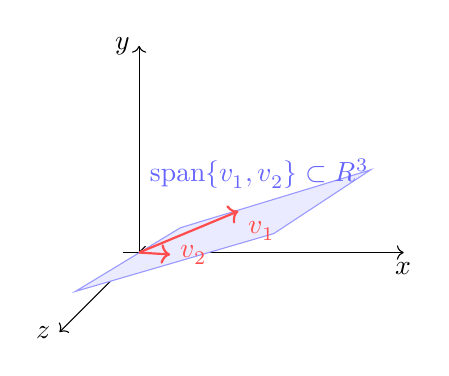
\begin{tikzpicture}[scale=1.05]
% axes
\draw[->] (-0.2,0,0) -- (3.2,0,0) node[below] {$x$};
\draw[->] (0,-0.2,0) -- (0,2.5,0) node[left] {$y$};
\draw[->] (0,0,-0.2) -- (0,0,2.5) node[left] {$z$};
% plane
\filldraw[fill=blue!8, draw=blue!40] (0.5,0.3,0) -- (2.8,1,0) -- (2.4,1,2) -- (0,0.3,2) -- cycle;
\node[blue!60] at (1.8,1.3,0.9) {$\operatorname{span}\{v_1,v_2\}\subset R^3$};
% vectors
\draw[->,thick,red!70] (0,0,0) -- (1.2,0.5,0) node[below right] {$v_1$};
\draw[->,thick,red!70] (0,0,0) -- (0.8,0.4,1.1) node[right] {$v_2$};
\end{tikzpicture}
\end{center}
\end{frame}


\begin{frame}{Proof of the Remark}
\begin{proof}[Proof of Remark 1]
Write $v=(\lambda_1,\dots,\lambda_n)^{\!\top}\in R^n$. Then
\[
Av=\lambda_1 c_1+\cdots+\lambda_n c_n\in \operatorname{span}\{c_1,\dots,c_n\}.
\]
Thus $\operatorname{Im}(A)\subseteq \operatorname{span}\{c_j\}$. Conversely, any linear combination $\sum \lambda_j c_j$ equals $A(\lambda_1,\dots,\lambda_n)^{\!\top}$, hence belongs to $\operatorname{Im}(A)$. Therefore, equality holds.
\end{proof}

\end{frame}

\begin{frame}{Proof of the Remark}

\begin{proof}[Proof of Remark 2]
Let $W:=\operatorname{span}\{v_1,\dots,v_m\}$.
If $w=\sum \lambda_i v_i$ and $w'=\sum \mu_i v_i$, then for any $a,b\in R$,
\[
aw+bw'=\sum (a\lambda_i + b\mu_i) v_i \in W,
\]
so $W$ is closed under linear combinations, hence under addition and $R$–scalar multiplication; thus $W$ is a submodule of $V$.
\end{proof}
\end{frame}


\begin{frame}{Example of a Span}
\vspace{-0.3cm}
\begin{block}{Polynomial Module}
Let $S=\{1,x,x^2\}\subseteq \mathbb{Q}[x]$. Then
\[
\operatorname{span}_{\mathbb{Q}}(S)
= \bigl\{\, a_0 + a_1 x + a_2 x^2 \mid a_0,a_1,a_2\in \mathbb{Q}\,\bigr\},
\]
which is the $\mathbb{Q}$–vector space (or $\mathbb{Q}$–module) of all quadratic polynomials.
\end{block}
\vspace{-0.3cm}
\textbf{Reasoning.}
\begin{itemize}
  \item Every quadratic polynomial $p(x)=a_0+a_1x+a_2x^2$ can be uniquely written as a linear combination of $1,x,x^2$.
  \item The set $\{1,x,x^2\}$ is linearly independent, since
  $c_0\!\cdot\!1 + c_1x + c_2x^2 = 0 \Rightarrow c_0=c_1=c_2=0$.
  \item Therefore, $\{1,x,x^2\}$ forms a \textbf{basis} of $\operatorname{span}_{\mathbb{Q}}(S)$.
\end{itemize}

\textbf{Interpretation.}
Geometrically, the span operation constructs the smallest subspace (submodule) of $\mathbb{Q}[x]$ that contains $S$.
\end{frame}



\begin{frame}{Definition and Notation}
Let $R$ be a CRWU, $V,W$ be $R$–modules, and $f:V\to W$ a function.

\begin{block}{Definition (Linear map / $R$–module homomorphism)}
$f$ is \textbf{linear} if for all $v_1,v_2\in V$ and $\lambda\in R$,
\begin{align*}
f(v_1+v_2)= &f(v_1)+f(v_2),\\
f(\lambda v)=&\lambda f(v).
\end{align*}
\end{block}

\begin{block}{Notation}
The set of all $R$–linear maps $V\to W$ is denoted
\[
\operatorname{Hom}_R(V,W)\quad \text{or}\quad \operatorname{Hom}(V,W)\quad \text{or}\mathcal{L}(V,W).
\]
\end{block}
\end{frame}

\begin{frame}{Examples of Linear Maps}
Let $R$ be a CRWU, $V,W$ be $R$–modules.
\begin{enumerate}
  \item \textbf{Zero map} $0:V\to W$, $0(v)=0$ is linear (both axioms hold trivially).
  \item \textbf{Identity} $\mathrm{id}_V:V\to V$ is linear.
  \item \textbf{Matrix map} If $V=R^n$, $W=R^m$ and $A\in M_{m\times n}(R)$, define $\mathcal A(v)=Av$. Then
  \[
  \mathcal A(v+w)=A(v+w)=Av+Aw,\qquad \mathcal A(\lambda v)=A(\lambda v)=\lambda (Av),
  \]
  so $\mathcal A$ is linear.
  \item \textbf{Integration} on $C^0[0,1]$: Let $V=W=C^0[0,1]$ over $R=\mathbb{R}$ and
  \[
  (I f)(x)=\int_0^x f(t)\,dt.
  \]
  Then $I$ is linear by linearity of the integral:
  \[
  I(f+g)=If+Ig,\qquad I(\lambda f)=\lambda (If).
  \]
\end{enumerate}
\end{frame}


\begin{frame}{Kernel - Image; Submodule Properties}

\begin{block}{Definitions}
Let $f\in \operatorname{Hom}_R(V,W)$.
\begin{align*}
    \ker f :=& \{\, v\in V \mid f(v)=0_W \,\}, \\
\operatorname{Im} f :=& \{\, f(v)\mid v\in V \,\} = \{\, w\in W \mid \exists v\in V,\ w=f(v)\,\}.
\end{align*}

\end{block}

\begin{block}{Proposition} Let $f\in \operatorname{Hom}_R(V,W)$. Then
$\ker f$ is a submodule of $V$, and $\operatorname{Im} f$ is a submodule of $W$.
\end{block}


\end{frame}

\begin{frame}{Kernel - Image; Submodule Properties}
\begin{block}{Proof}
If $u,v\in \ker f$ and $\lambda,\mu\in R$, then
\[
f(\lambda u+\mu v)=\lambda f(u)+\mu f(v)=0,
\]
so $\lambda u+\mu v\in\ker f$. Thus $\ker f\le V$.

If $y_1=f(v_1), y_2=f(v_2)$ and $\lambda,\mu\in R$, then
\[
\lambda y_1+\mu y_2=\lambda f(v_1)+\mu f(v_2)=f(\lambda v_1+\mu v_2)\in \operatorname{Im} f.
\]
Hence $\operatorname{Im} f\le W$.
\end{block}
\end{frame}


\begin{frame}{Example}
\vspace{-0.3cm}
Let $R=\mathbb{R}$ and
\[
V=W=\{\, a_0+a_1 x+a_2 x^2 \mid a_0,a_1,a_2\in\mathbb{R}\,\},
\]
define $D:V\to V$ by $Df=f'$.

\textbf{Computations}
\[
D(2+4x+x^2)=4+2x.
\]
\[
\ker D=\{\, a_0 \mid a_0\in\mathbb{R}\,\} \quad (\text{constant polynomials}),
\]
\[
\operatorname{Im} D=\{\, a_0+a_1 x \mid a_0,a_1\in\mathbb{R}\,\} \quad (\text{linear polynomials}).
\]


\begin{proof}[Justification]
$Df=0$ iff $f$ is constant, hence $\ker D$ are the constants. If $f=a_0+a_1x+a_2 x^2$, then $Df=a_1+2a_2 x$ is any linear polynomial: given $\alpha+\beta x$ choose $a_1=\alpha$, $a_2=\beta/2$. Thus the image equals the set of linear polynomials.
\end{proof}
\end{frame}


\begin{frame}{Matrix Image as Span of Columns}

\begin{center}
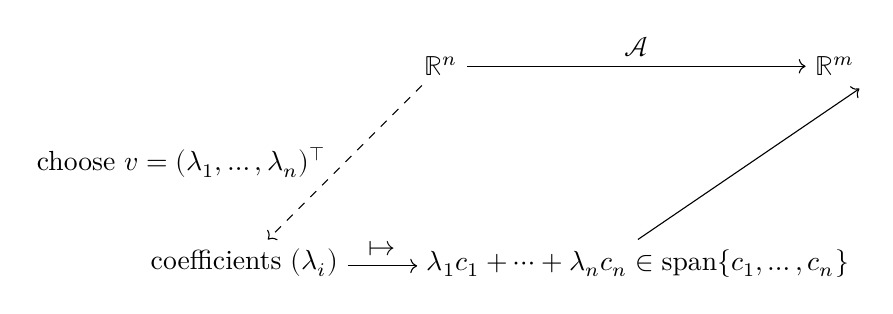
\begin{tikzpicture}[
    % Removed 'node distance' since we are using explicit coordinates
    every node/.style={font=\normalsize} % Consistent font size for nodes
]
    % Define the nodes using (x, y) coordinates
    \node (Rn) at (0, 0) {$\mathbb{R}^n$};
    % Position is down and left from Rn
    \node (Coeff) at (-2.5, -2.5) {$\text{coefficients } (\lambda_i)$};
    % Position is right of Rn
    \node (Rm) at (5, 0) {$\mathbb{R}^m$};
    % Position is right of Coeff
    \node (Span) at (2.5, -2.5) [align=left]
        {$\lambda_1 c_1+\cdots+\lambda_n c_n \in \operatorname{span}\{c_1,\dots,c_n\}$};

    % 1. R^n to R^m (Right Arrow: \mathcal{A})
    \draw[->] (Rn) -- node[above] {$\mathcal A$} (Rm);

    % 2. R^n to Coefficients (Down-Left Arrow: dashed, label below)
    \draw[->, dashed] (Rn) -- (Coeff)
        node[midway, left, align=center] {
            $\text{choose }v=(\lambda_1,\dots,\lambda_n)^\top$
        };

    % 3. Coefficients to Span (Right Arrow: mapsto)
    \draw[->, transform canvas={yshift=-1pt}] (Coeff) -- (Span)
        node[midway, above] {$\mapsto$};

    % 4. Span to R^m (Up-Right Arrow: inclusion)
    % Connecting from the top of Span to the bottom-right of Rm
    \draw[->, shorten >= 2pt] (Span.north) -- (Rm.south east);

\end{tikzpicture}
\end{center}
\[
\operatorname{Im}(\mathcal A)=\operatorname{span}\{c_1,\dots,c_n\}\subseteq R^m.
\]
\end{frame}


\begin{frame}{Proposition: $f$ injective $\iff \ker f=\{0\}$}
\begin{block}{Proposition.}
Let $R$ be a CRWU, $V,W$ be $R$–modules, and $f\in\operatorname{Hom}_R(V,W)$. Then
\[
f \text{ is injective } \iff \ker f=\{0\}.
\]
\end{block}

\begin{proof}
($\Rightarrow$) If $f$ is injective and $v\in\ker f$, then $f(v)=0=f(0)$, hence $v=0$. So $\ker f=\{0\}$.

($\Leftarrow$) Suppose $\ker f=\{0\}$ and $f(v_1)=f(v_2)$. Then $f(v_1-v_2)=0$, so $v_1-v_2\in\ker f$, hence $v_1-v_2=0$, i.e.\ $v_1=v_2$. Thus $f$ is injective.
\end{proof}
\end{frame}


\begin{frame}{Definition and Equivalent Characterization}
\begin{block}{Definition (Isomorphism).}
Let $R$ be a CRWU, $V,W$ $R$–modules, and $f\in\operatorname{Hom}_R(V,W)$. We say $f$ is an \emph{isomorphism} if there exists $g\in\operatorname{Hom}_R(W,V)$ such that
\[
g\circ f=\mathrm{id}_V,\qquad f\circ g=\mathrm{id}_W.
\]
\end{block}
\begin{block}{Equivalently}
$f$ is bijective. In this case $V$ and $W$ are \emph{isomorphic}, written $V\cong W$.
\end{block}
\end{frame}

\begin{frame}{Flattening Matrices is an Isomorphism}
Let $R$ be a CRWU and $m,n\in\mathbb{N}$. Put $V=M_{m\times n}(R)$ and $W=R^{mn}$. Define
\[
F:V\to W,\quad
F\!\left(\begin{bmatrix}
a_{11} & a_{12} & \cdots & a_{1n}\\
a_{21} & a_{22} & \cdots & a_{2n}\\
\vdots & \vdots & \ddots & \vdots\\
a_{m1} & a_{m2} & \cdots & a_{mn}
\end{bmatrix}\right)
=
\begin{pmatrix}
a_{11}\\ a_{12}\\ \vdots\\ a_{1n}\\ a_{21}\\ \vdots\\ a_{2n}\\ \vdots\\ a_{m1}\\ \vdots\\ a_{mn}
\end{pmatrix}
\in R^{mn}.
\]
\end{frame}

\begin{frame}{Flattening Matrices is an Isomorphism}
\vspace{-0.3cm}
\begin{block}{Claim:} $F$ is a linear isomorphism.
\end{block}
\vspace{-0.3cm}
\begin{block}{Linearity:} $F(A+B)=F(A)+F(B)$ and $F(\lambda A)=\lambda F(A)$ hold entrywise.
\end{block}
\vspace{-0.3cm}
\begin{block}{Injective:} $F(A)=0$ implies all $a_{ij}=0$, hence $A=0$.
\end{block}
\begin{block}{Surjective:} Given $(b_1,\dots,b_{mn})^\top\in R^{mn}$, place entries row-by-row into a matrix $B$; then $F(B)=(b_1,\dots,b_{mn})^\top$.

Therefore $F$ is a linear bijection, i.e.\ an isomorphism $M_{m\times n}(R)\cong R^{mn}$.
\end{block}

\end{frame}

\begin{frame}{Universal Property of Free Modules}
\begin{block}{Proposition (Extension from a basis).}
Let $R$ be a CRWU, $V$ a free $R$–module with basis $S=\{e_1,\dots,e_n\}$ (possibly infinite index set), $W$ an $R$–module, and pick arbitrary $w_1,\dots,w_n\in W$. Then there exists a unique linear map $f\in\operatorname{Hom}_R(V,W)$ such that
\[
f(e_i)=w_i,\quad i=1,\dots,n.
\]

\end{block}
\end{frame}

\begin{frame}{Proof}

\begin{proof}
Every $v\in V$ can be written uniquely as $v=\sum_{i=1}^n \lambda_i e_i$ with $\lambda_i\in R$ (finite sum if $S$ infinite).
Define $f(v):=\sum_{i=1}^n \lambda_i w_i$. This is well-defined by uniqueness of the coefficients.
For linearity: if $v=\sum\lambda_i e_i$ and $u=\sum\mu_i e_i$, then
\[
f(v+u)=\sum (\lambda_i+\mu_i)w_i = \sum \lambda_i w_i + \sum \mu_i w_i = f(v)+f(u),
\]
and $f(\alpha v)=\sum (\alpha\lambda_i) w_i=\alpha \sum \lambda_i w_i=\alpha f(v)$. By construction $f(e_i)=w_i$.

Uniqueness: if $g$ is another linear map with $g(e_i)=w_i$, then for any $v=\sum \lambda_i e_i$,
$g(v)=\sum \lambda_i g(e_i)=\sum \lambda_i w_i=f(v)$. Hence $g=f$.
\end{proof}


\end{frame}

\begin{frame}{Example}
\begin{block}{$R^n \cong \mathrm{Free}_R(S)$}
    Let $R$ be a CRWU, $n\in\mathbb{N}$, and $S=\{e_1,\dots,e_n\}$ a finite set. Define
\[
f:R^n\to \mathrm{Free}_R(S),\qquad
f(1,0,\dots,0)=e_1,\ \dots,\ f(0,\dots,0,1)=e_n,
\]
and extend $R$–linearly. Then for $(\lambda_1,\dots,\lambda_n)\in R^n$,
\[
f(\lambda_1,\dots,\lambda_n)=\lambda_1 e_1+\cdots+\lambda_n e_n.
\]
By the previous proposition, $f$ is linear and bijective (its inverse sends $\sum \lambda_i e_i$ to $(\lambda_1,\dots,\lambda_n)$). Hence $R^n\cong \mathrm{Free}_R(S)$.
\end{block}
\end{frame}

%============================================================
\section{Coordinate Isomorphism}
%============================================================

\begin{frame}{Coordinate Map with Respect to a Basis}
Let $R$ be a CRWU and $V$ a finite-dimensional $R$–module with ordered basis $e=(e_1,\dots,e_n)$.

\textbf{Definition (Coordinates).}
For $v\in V$ written uniquely as $v=\lambda_1 e_1+\cdots+\lambda_n e_n$, define
\[
(\cdot)^e: V\to R^n,\qquad v^e:=(\lambda_1,\dots,\lambda_n)^\top.
\]

\textbf{Proposition.} $(\cdot)^e$ is a linear isomorphism.

\begin{proof}
Linearity is immediate from linearity of coordinate extraction. Injectivity: $v^e=0$ implies all coordinates $=0$, hence $v=0$. Surjectivity: given $(\mu_1,\dots,\mu_n)^\top$, take $v=\sum \mu_i e_i$, then $v^e=(\mu_1,\dots,\mu_n)^\top$.
\end{proof}
\end{frame}

\begin{frame}{Example}

\textbf{Setup.}
Let $V = \{\, a_0 + a_1x + a_2x^2 \mid a_0,a_1,a_2 \in R \,\}$ be the $R$–module (or vector space, if $R$ is a field) of quadratic polynomials,
and let $e = (1, x, x^2)$ be its ordered basis.

\begin{block}{Coordinate Map}
Every element $v \in V$ can be uniquely written as
\[
v = a_0\cdot 1 + a_1\cdot x + a_2\cdot x^2,
\]
so its coordinate vector with respect to $e$ is
\[
v^e =
\begin{pmatrix}
a_0\\[4pt]
a_1\\[4pt]
a_2
\end{pmatrix}
\in R^3.
\]
\end{block}

\end{frame}

\begin{frame}{Example}
\vspace{-0.3cm}
\begin{block}{Interpretation.}
\begin{itemize}
  \item The coordinate map $(\cdot)^e : V \to R^3$ translates each polynomial into its list of coefficients.
  \item It is a linear isomorphism — addition and scalar multiplication of polynomials correspond exactly to those of their coordinate vectors:
  \[
  (p+q)^e = p^e + q^e, \qquad (\lambda p)^e = \lambda p^e.
  \]
  \item Hence $V$ is \emph{algebraically identical} to $R^3$ under this basis, just viewed in a different “language” — coefficients instead of components.
\end{itemize}

\textbf{Visualization.}
Think of the polynomial $a_0+a_1x+a_2x^2$ as a point in $R^3$ whose coordinates are $(a_0,a_1,a_2)$ — the space of all quadratic shapes parameterized by their coefficients.
\end{block}

\end{frame}


\begin{frame}{Hom is a Submodule of $W^V$}
\begin{block}{Definition}
    Let $W^V$ denote all functions $V\to W$ with pointwise operations:
\begin{align*}
(f+g)(v):=&f(v)+g(v),\\ (\lambda f)(v):=&\lambda f(v).
\end{align*}
\end{block}
\begin{block}{Proposition.} $\operatorname{Hom}_R(V,W)\subseteq W^V$ is a submodule (closed under $+$ and $R$–scalars).
\end{block}

\end{frame}

\begin{frame}{Hom is a Submodule of $W^V$}
\begin{proof}
If $f,g\in\operatorname{Hom}_R(V,W)$ and $\lambda\in R$, for any $v,u\in V$:
\begin{align*}
(f+g)(v+u)=&f(v+u)+g(v+u)=f(v)+f(u)+g(v)+g(u)\\
=&(f+g)(v)+(f+g)(u),
\end{align*}
\[
(f+g)(\alpha v)=f(\alpha v)+g(\alpha v)=\alpha f(v)+\alpha g(v)=\alpha (f+g)(v).
\]
So $f+g$ is linear.

Similarly $(\lambda f)(v+u)=\lambda f(v+u)=\lambda f(v)+\lambda f(u)$ and $(\lambda f)(\alpha v)=\lambda \alpha f(v) = \alpha(\lambda f)(v)$, hence $\lambda f$ is linear.

Therefore $\operatorname{Hom}_R(V,W)$ is an $R$–submodule of $W^V$.
\end{proof}
\end{frame}

\begin{frame}{Example in $\mathbb{R}$}
\vspace{-0.3cm}
\begin{block}{$h=2D-3\,\mathrm{id}$ on Quadratics}
    Let $R=\mathbb{R}$ and $V=\{a_0+a_1 x+a_2 x^2\}$ with basis $e=(1,x,x^2)$. Put
\[
f=D,\quad g=\mathrm{id}_V,\quad h=2f-3g.
\]
Then for $p(x)=a_0+a_1 x+a_2 x^2$,
\begin{align*}
h(p)=&2(a_1+2a_2 x)-3(a_0+a_1 x+a_2 x^2)\\
=&(-3a_0+2a_1)\;+\;(-3a_1+4a_2)x\;+\;(-3a_2)x^2.
\end{align*}
In coordinates $p^e=(a_0,a_1,a_2)^\top$,
\[
h^e(p)=\begin{pmatrix}-3a_0+2a_1\\ -3a_1+4a_2\\ -3a_2\end{pmatrix}.
\]
\end{block}
\end{frame}


\begin{frame}{Matrix of a Linear Map}
\begin{block}{}
    Let $V,W$ be finite-dimensional $R$–modules, with ordered bases
\[
e=(e_1,\dots,e_n) \text{ for } V,\qquad f=(f_1,\dots,f_m) \text{ for } W.
\]
For $\mathcal{A}\in\operatorname{Hom}_R(V,W)$, write for each $1\le j\le n$:
\[
\mathcal{A}(e_j)=a_{1j}f_1+\cdots+a_{mj}f_m.
\]
\textbf{Definition.} The matrix of $\mathcal{A}$ w.r.t.\ $(e,f)$ is
\[
(\mathcal{A})_e^f =
\begin{bmatrix}
a_{11} & a_{12} & \cdots & a_{1n}\\
a_{21} & a_{22} & \cdots & a_{2n}\\
\vdots & \vdots & \ddots & \vdots\\
a_{m1} & a_{m2} & \cdots & a_{mn}
\end{bmatrix}\in M_{m\times n}(R).
\]
\end{block}
\end{frame}

\begin{frame}{Example}
\begin{block}{Matrix of $h=2D-3\,\mathrm{id}$}
    With $e=f=(1,x,x^2)$ and the computations
\[
h(1)=-3,\qquad h(x)=2-3x,\qquad h(x^2)=4x-3x^2,
\]
their coordinate columns (w.r.t.\ $e$) are
\[
[-3,0,0]^\top,\quad [2,-3,0]^\top,\quad [0,4,-3]^\top.
\]
Hence
\[
(h)_e^f=
\begin{bmatrix}
-3 & 2 & 0\\
0  & -3 & 4\\
0  & 0  & -3
\end{bmatrix}.
\]
\end{block}

\end{frame}


\begin{frame}{Composition Corresponds to Matrix Product}
Let $U,V,W$ be finite-dimensional $R$–modules with ordered bases
\[
e=(e_1,\dots,e_p),\quad f=(f_1,\dots,f_m),\quad g=(g_1,\dots,g_n).
\]
Let $A\in\operatorname{Hom}_R(U,V)$ and $B\in\operatorname{Hom}_R(V,W)$. Then $B\circ A\in\operatorname{Hom}_R(U,W)$ and
\[
(A)_e^f\in M_{m\times p}(R),\quad (B)_f^g\in M_{n\times m}(R),\quad (B\circ A)_e^g\in M_{n\times p}(R),
\]
with the identity
\[
(B\circ A)_e^g=(B)_f^g\,(A)_e^f.
\]
\begin{center}
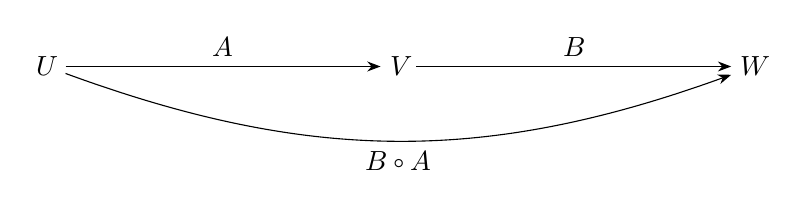
\begin{tikzpicture}[
    node distance=4cm,
    >=Stealth,
    every node/.style={font=\normalsize}
]
    % Define nodes
    \node (U) {$U$};
    \node (V) [right=4cm of U] {$V$};
    \node (W) [right=4cm of V] {$W$};

    % Draw arrows
    \draw[->] (U) -- node[above] {$A$} (V);
    \draw[->] (V) -- node[above] {$B$} (W);
    \draw[->, bend right=20] (U) to node[below] {$B\circ A$} (W);
\end{tikzpicture}
\end{center}

\end{frame}

\begin{frame}{Proof}
    \begin{proof}
For each $j$, write $A(e_j)=\sum_{i=1}^m \alpha_{ij} f_i$ and $B(f_i)=\sum_{k=1}^n \beta_{ki} g_k$.
Then
\begin{align*}
    (B\circ A)(e_j)=&B\Big(\sum_i \alpha_{ij} f_i\Big)=\sum_i \alpha_{ij} \Big(\sum_k \beta_{ki} g_k\Big)\\
=&\sum_k \Big(\sum_i \beta_{ki}\alpha_{ij}\Big) g_k.
\end{align*}

Thus the $(k,j)$–entry of $(B\circ A)_e^g$ is $\sum_i \beta_{ki}\alpha_{ij}$, i.e.\ the matrix product $(B)_f^g (A)_e^f$.
\end{proof}
\end{frame}

\begin{frame}{Summary}
\begin{itemize}
  \item Defined free and finite–dimensional $R$–modules; proved dimension is well–defined for finite-dimensional modules (IBN via reduction mod maximal ideals).
  \item Computed dimensions of $R^n$, $M_{m\times n}(R)$, $\mathbf{0}$, and $R[x]$.
  \item Defined span; proved image of a matrix equals the span of its columns; proved span is a submodule.
  \item Defined linear maps; verified linearity in key examples (zero, identity, matrix, integral).
  \item Defined kernel and image; proved they are submodules; computed them for $D$ on quadratics.
\end{itemize}
\end{frame}

\begin{frame}{Thanks}
  \cmcendframe
\end{frame}

\end{document}
